\chapter{Figures and Tables}

Figures and tables are referred to as floats in the {\TeX} world. These are
elements which cannot be broken across pages. For more details on these, refer
to the relevant chapter of the tutorial.
%
%
%
%
\section{Figures}
A simple figure is shown below:

\begin{figure}[h]
\centering

\includegraphics[width=0.25\textwidth]{tux}
\label{fig:tux}
\caption{This is a photo of Tux. He is a very friendly penguin. We will meet
his friends shortly.}
\end{figure}

As with almost all other elements in {\LaTeX} figures too can be
cross-referenced using the labels. Make sure to provide these for all figures
and choose a descriptive tag while doing so. That way, later on if one needs to
refer to the figure, there is no need for hunting around to find where the
image is. Instead, Overleaf will automatically suggest a list of tags to
choose from while invoking the {\ttfamily \textbackslash ref} command.

Since floats are complex, one does not have very fine-grained control over the
location of its placement relative to surrounding text. While preparing a
document, the author should not be too concerned about the placement unless it
is severely out of place. Instead, once the document is near-complete, fine
tuning can be done to precise measurements if desired/possible. Otherwise, some
fine-tuning might go to waste as significant changes to the document (and hence
the layout of the material) occurs.

The recommended way to place multiple figures is by use of the
{\ttfamily subcaption} package. Make sure to include this.
An example is shown in figure \ref{fig:tux-with-friends}.

\begin{figure}
    \subfloat[Tux]{
        
\includegraphics[width=0.2\textwidth]{tux}
        \label{fig:m-tux}
    }
    \hfill
    \subfloat[Adiumy]{
        
\includegraphics[width=0.2\textwidth]{adiumy}
        \label{fig:m-adiumy}
    }
    \hfill
    \subfloat[GNU Head]{
        
\includegraphics[width=0.2\textwidth]{gnuhead}
        \label{fig:m-gnuhead}
    }
    \hfill
    \subfloat[Emule]{
        
\includegraphics[width=0.2\textwidth]{emule}
        \label{fig:m-emule}
    }
    \hfill
    \par
    \subfloat[Konqi]{
        
\includegraphics[width=0.2\textwidth]{konqi}
        \label{fig:m-konqi}
    }
    \hfill
    \subfloat[Katie]{
        
\includegraphics[width=0.2\textwidth]{katie}
        \label{fig:m-katie}
    }
    \hfill
    \subfloat[Wiber]{
        
\includegraphics[width=0.2\textwidth]{wiber}
        \label{fig:m-wiber}
    }
    \hfill
    \subfloat[Camelia]{
        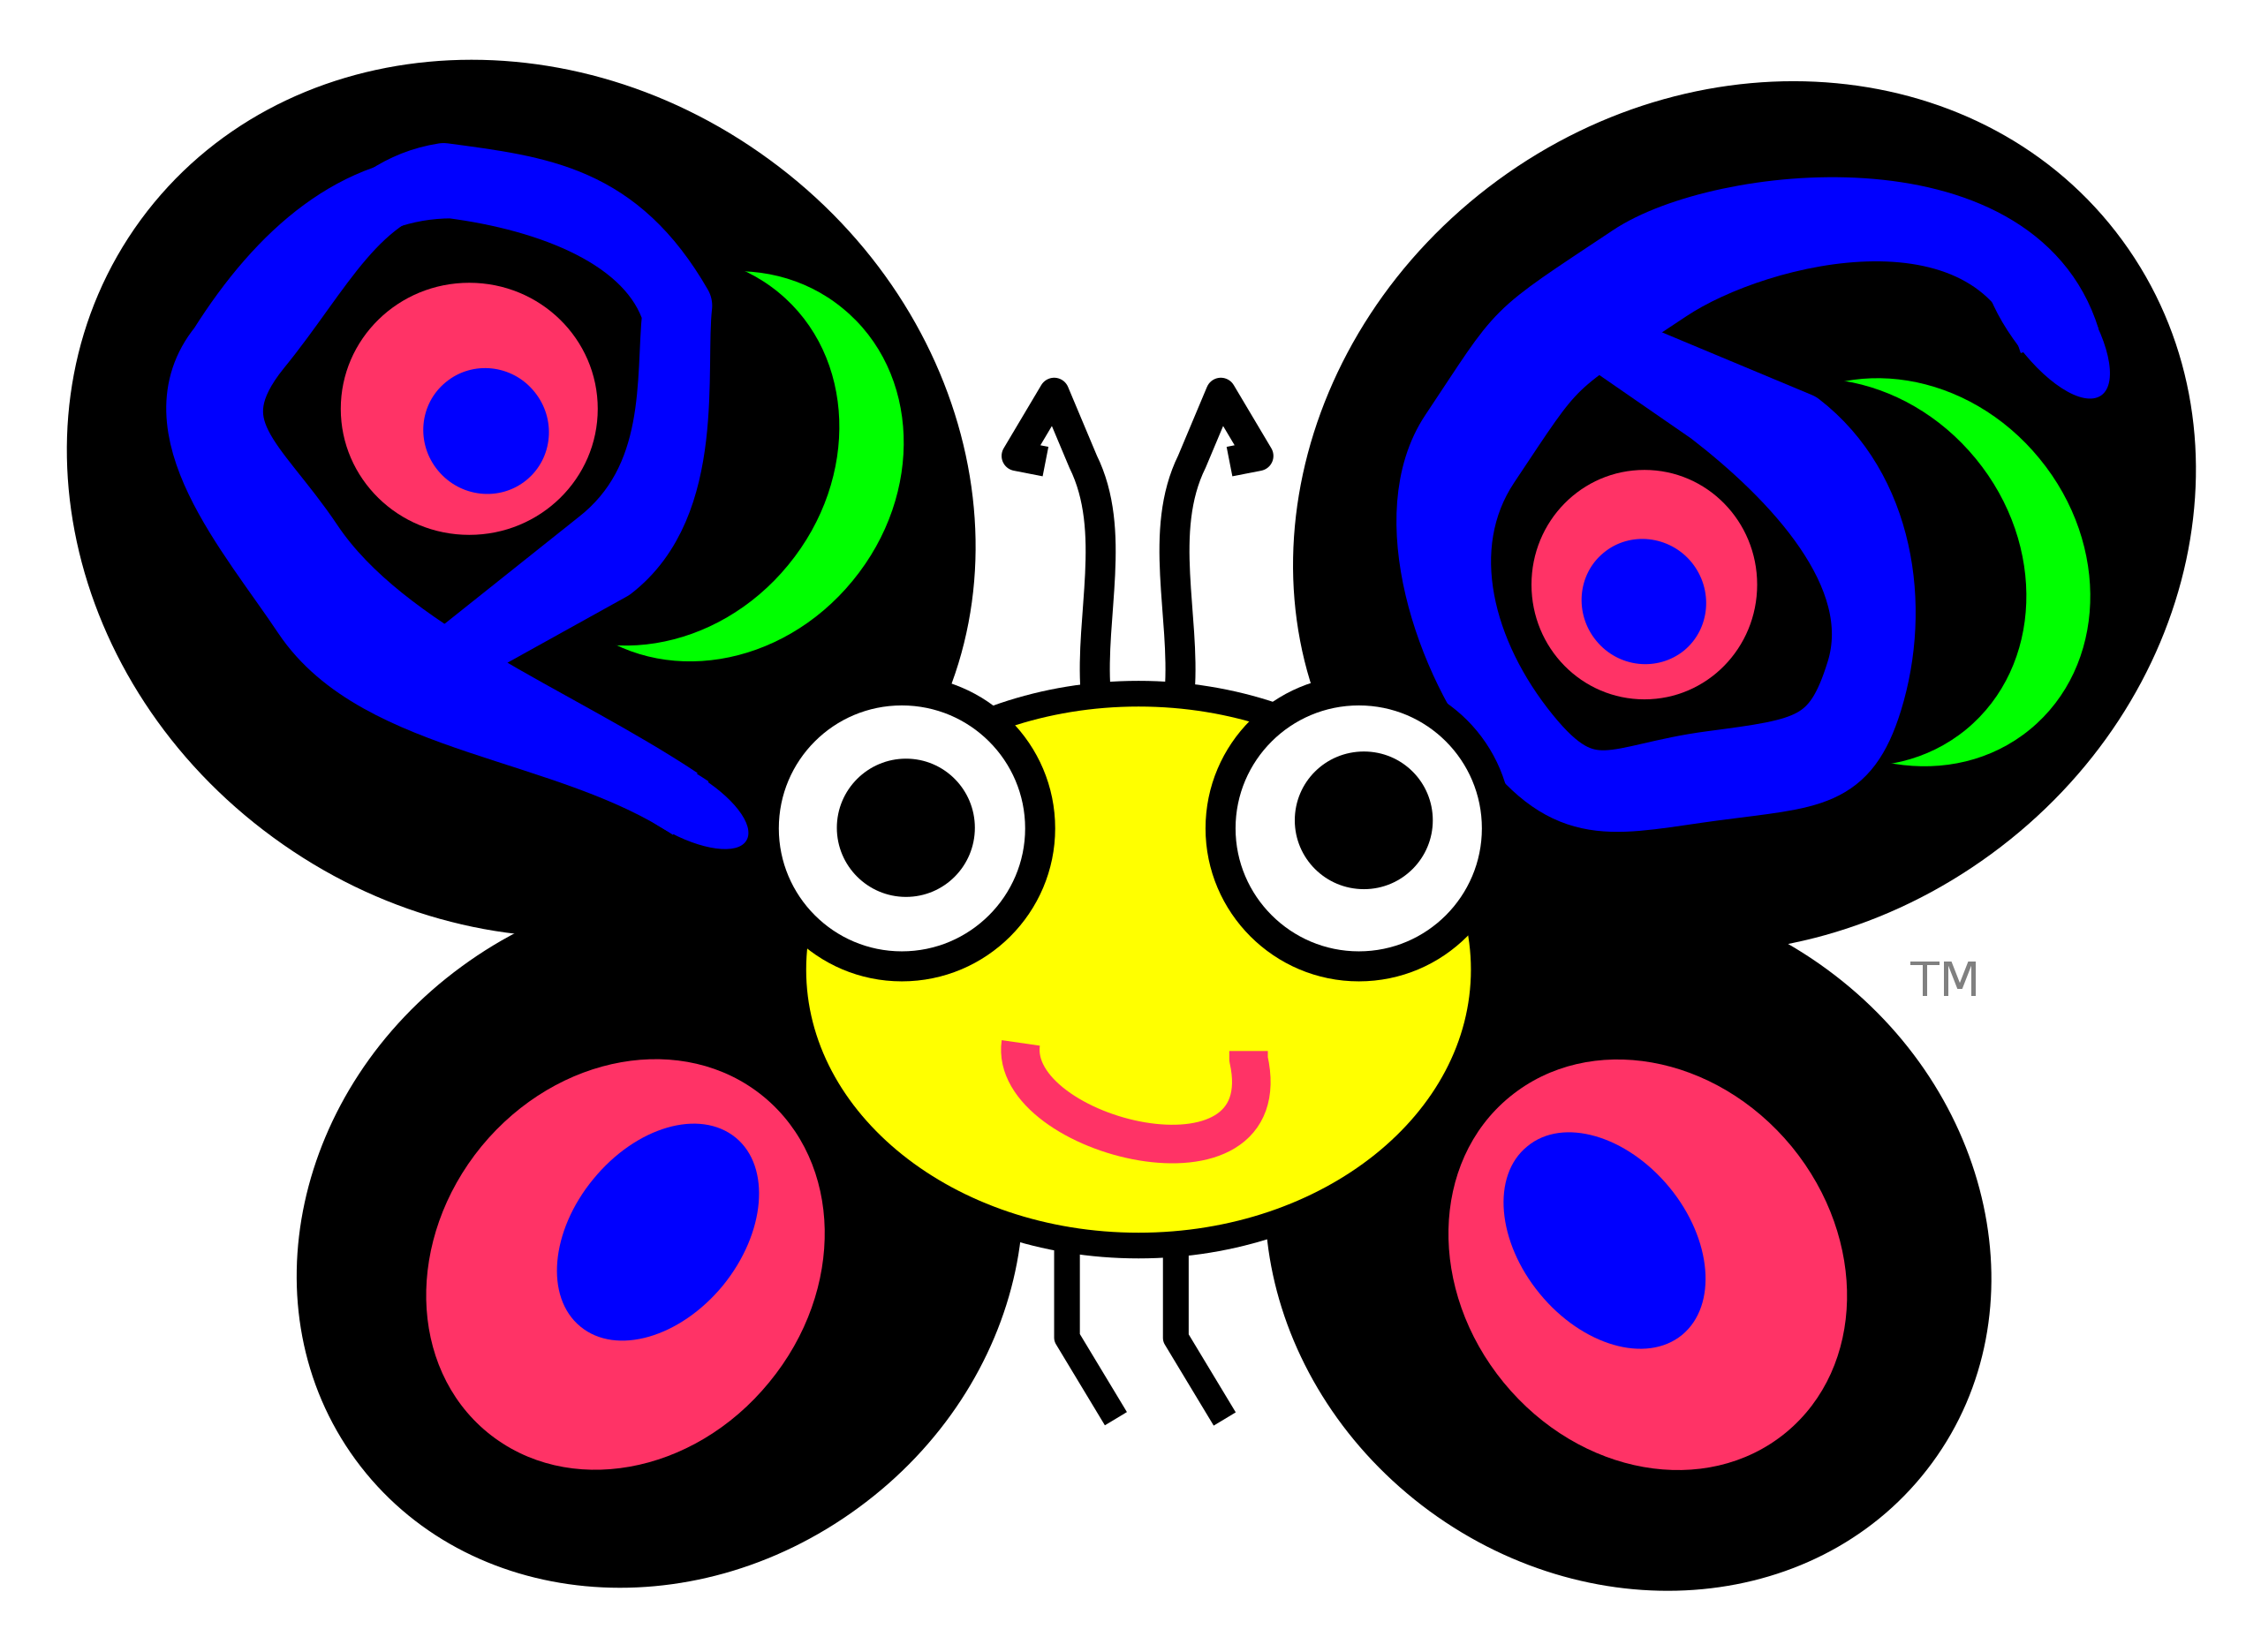
\includegraphics[width=0.2\textwidth]{camelia}
        \label{fig:m-camelia}
    }
\caption{Tux with his various friends. Notice that captions of figures are
placed below the figure and are properly line spaced as per the guidelines}
\label{fig:tux-with-friends}
\end{figure}
%
%
%
%
\section{Tables}
Please refer to the tutorial for a slightly detailed note about tables. A
simple table is shown below.
\begin{table}
    \captionabove{Shown below is a simple elegant table with a
    very long caption. Tables are quite helpful in
    organizing information in a presentable manner.}
    \centering
    \begin{tabular}{ll}
        \toprule
        \textbf{Table} & \textbf{Head}  \\
        \midrule
        stuff & stuff \\
        stuff & stuff \\
        stuff & stuff \\
        stuff & stuff \\
        stuff & stuff \\
        \bottomrule
    \end{tabular}
\label{tab:elegant-table}
\end{table}
Table captions are placed above the table. They are line-spaced as per the
guidelines. It is not recommended to break paragraphs after a table unless
absolutely necessary. Note that {\ttfamily \textbackslash captionabove}  
(not {\ttfamily \textbackslash caption}), is used to place captions in tables. 
Only then will the spacing around the captions of tables be appropriate. Make 
note of this fact.

Far more complex table layouts are possible using {\ttfamily multicolumn}
and/or specifying different column types for the {\ttfamily tabular} block.
Refer to the tutorial for more details. An example is shown below:

\begin{table}
\centering
\captionabove{A complex table is shown here. Careful use of the column specifiers
along with thoughtful (re)organization of the material can yield great results}
\begin{tabular}{>{\bfseries}p{2cm} rrrr}
\toprule
& \multicolumn{2}{c}{\textbf{Value}}
& \multicolumn{2}{c}{\textbf{Profit}} \\
\cmidrule(lr){2-3} \cmidrule(lr){4-5}
  Aspect
& \multicolumn{1}{c}{Before 2019}
& \multicolumn{1}{c}{After 2019}
& \multicolumn{1}{c}{Before 2020}
& \multicolumn{1}{c}{After 2020}      \\
\midrule
  Whatever
& 30
& 40
& 20
& 2       \\
  Aspect
& 33
& 45
& 10
& 5       \\
  Entries
& 37
& 51
& 90
& 600     \\
  Here
& 33
& 67
& 97
& 52      \\
\bottomrule
\end{tabular}
\end{table}

Further, the {\ttfamily multirow} functionality offered by the {\ttfamily
 multirow} package is sometimes useful. The same example as above is repeated
below with a slight change using the {\ttfamily multirow} functionality

\begin{table}
\centering
\captionabove{A complex table is shown here. Sometimes, one might need to have cell
entries which span more than a single row; this too is possible as shown below}
\begin{tabular}{>{\bfseries}p{2cm} rrrr}
\toprule
  \multirow{2}[3]{*}{Aspect}
& \multicolumn{2}{c}{\textbf{Value}}
& \multicolumn{2}{c}{\textbf{Profit}} \\
\cmidrule(lr){2-3} \cmidrule(lr){4-5}
& \multicolumn{1}{c}{Before 2019}
& \multicolumn{1}{c}{After 2019}
& \multicolumn{1}{c}{Before 2020}
& \multicolumn{1}{c}{After 2020}      \\
\midrule
  Whatever
& 30
& 40
& 20
& 2       \\
  Aspect
& 33
& 45
& 10
& 5       \\
  Entries
& 37
& 51
& 90
& 600     \\
  Here
& 33
& 67
& 97
& 52      \\
\bottomrule
\end{tabular}
\end{table}

Bear in mind that as in the case of figures, the tables too cannot always be
precisely positioned as desired. Fine-tuning of the positioning by the use of
position specifiers is best left to the final stages of the document
preparation.

Finally, vertical rules in tables are not only unsightly, but also largely
unnecessary (for most cases). If one still wants properly positioned vertical
rules in tables, refer to the tutorial file for more information.
%
%
%
%
\section{Bibliography References}
{Bib\TeX} is the only supported mechanism to manage bibliography and citations.
For those unfamiliar with Bib\TeX, several useful tutorials are available on
the internet.

In nutshell, one requires a {\ttfamily references.bib} file containing all the
relevant details of the material to be referenced in the {Bib\TeX} format. Make
sure to the {\ttfamily references.bib} file is free of any errors to ensure
that the bibliography is typeset correctly. Many popular reference management
tools support {Bib\TeX} export of libraries.

With that in place one simply uses the {\ttfamily \textbackslash cite} command
along with the tag of the entry to be referenced. For instance, this is a very
nice paper \cite{Stroock_Varadhan_1971}. While we are on the topic, let me
recommend another classic: \cite{Nash_1951}. Or perhaps, some other favorites
might interest you if you work in related fields: see \cite{Chernoff_1972},
\cite{Wald_2004}, \cite{Zhang_2014} or \cite{Shannon_1948} for a nice
selection. It is also worth mentioning that the work of
\cite{Polyanskiy_Poor_Verdu_2010} is well regarded.